% Figure 18 -- a) Type IV SCFT Newton polygon, b) Type II SCFT Newton polygon
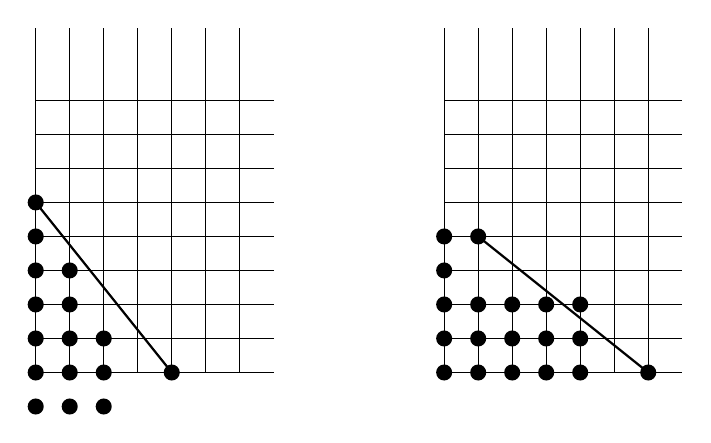
\begin{tikzpicture}[x=1pt,y=1pt,>=stealth,line width=0.5pt]
  \def\u{12.29}
  % ===================== panel a) =====================
  \foreach \i in {0,...,6} {\draw[line width=0.4pt] ({\i*\u},0) -- ({\i*\u},124.4);}
  \foreach \j in {0,...,8} {\draw[line width=0.4pt] (0,{\j*\u}) -- ({7*\u},{\j*\u});}
  \draw[line width=0.8pt] (0,{5*\u}) -- ({4*\u},0);
  \foreach \i/\j in {0/5,0/4,0/3,1/3,0/2,1/2,0/1,1/1,2/1,0/0,1/0,2/0,4/0,0/-1,1/-1,2/-1}
    {\fill ({\i*\u},{\j*\u}) circle[radius=2.9pt];}
  % ===================== panel b) =====================
  \begin{scope}[xshift=147.6pt]
    \foreach \i in {0,...,6} {\draw[line width=0.4pt] ({\i*\u},0) -- ({\i*\u},124.4);}
    \foreach \j in {0,...,8} {\draw[line width=0.4pt] (0,{\j*\u}) -- ({7*\u},{\j*\u});}
    \draw[line width=0.8pt] ({\u},{4*\u}) -- ({6*\u},0);
    \foreach \i/\j in {0/4,1/4,0/3,0/2,1/2,2/2,3/2,4/2,0/1,1/1,2/1,3/1,4/1,0/0,1/0,2/0,3/0,4/0,6/0}
      {\fill ({\i*\u},{\j*\u}) circle[radius=2.9pt];}
  \end{scope}
\end{tikzpicture}
